\documentclass[a4paper,12pt]{report} % Format du papier, type de document
 
\usepackage[utf8]{inputenc} % Permet de tapper les accents tels quels
\usepackage[T1]{fontenc} % Permet l'utilisation d'accents
\usepackage[french]{babel} % Dit que le document est en français
\usepackage{amsfonts} % Différents packages... Lire la doc....
\usepackage{amsmath}
\usepackage{listings}
\usepackage{color}
\usepackage{graphicx} %affichage d'image
\usepackage{moreverb}
\usepackage[colorlinks=true,linkcolor=blue]{hyperref} %lien hypertexte
\usepackage[all]{hypcap}
\usepackage{fullpage}
\usepackage{fancyhdr}
\pagestyle{fancy}
\renewcommand{\thesection}{\arabic{section}}
\setcounter{tocdepth}{5}
\setcounter{secnumdepth}{5}

\renewcommand{\headrulewidth}{0pt} 
\fancyhead{} %retire en tete

\renewcommand{\footrulewidth}{1pt} %bas de page
\fancyfoot[C]{\textbf{\thepage}} 
\fancyfoot[L]{Software evolution}
\fancyfoot[R]{Jpacman framework}

\title{Software evolution \\ JPacman framework}
\author{Ducruet Corentin \\ Gallois Florent \\ Ledru Santorin}
\date{Année académique\\2015 - 2016}
%\begin{figure}[!h] %on ouvre l'environnement figure
%		\centering
%		\includegraphics[width=108mm,height=65mm]{impulsion.png}
%	\end{figure} 

%\begin{figure}%[H] si on veut que l image soit a cet endroit
%	\centering
%	\includegraphics[width=108mm,height=65mm]{./scr/logo}
%	\caption{Icône}
%	\label{fig:Icône}
%\end{figure}

\begin{document} 
\maketitle
\newpage 
\addtocontents{toc}{\protect\thispagestyle{fancy}} %modifie mise en page table des matiere
\tableofcontents
\newpage
%\raggedright
\section{Introduction}
Dans le cadre du cours de Softare Evolution, nous devons mettre en pratique les concepts d'évolution logicielle vus en cours. Le projet qui nous est confié consiste à récupérer un projet de pacman et d'y implémenter plusieurs fonctionnalités. Ces mêmes fonctionnalités doivent être faites tout en suivant un processus de développement dirigé par les tests . Après la réalisation de ces tâches, il nous est demandé de rassembler ces différents travaux dans le logiciel. Enfin, une analyse de la qualité ainsi qu'une amélioration du code doit nous permettre de terminer le logiciel.
Dans un premier temps, nous étudierons chaque tâche individuelle : dans un premier temps nous parlerons de la réalisation de la supergomme, puis de la série de labyrinthe et enfin l'implémentation de l'IA des fantômes.
Dans un deuxième temps, nous parlerons des difficultés rencontrés lors du merge des trois fonctionnalités et enfin nous parlerons de l'analyse du code et des améliorations.

\section{Supergomme - Ducruet Corentin}
\subsection{Programme initial et objectifs}
Dans la version de initial du framework Jpacman, il n'y avais qu'un seul type de gomme qui avait pour seul effet d'augmenter notre score de 10 points. Il nous a été demandé d'ajouter la fonctionnalité "Supergomme". Cette fonctionnalité ajoute un nouveau type de gomme (les "Supergomme"). celles-ci se distinguent des autres gommes par leur effet. Tout d'abord, elles sont rouges pour pouvoir les différentier visuellement. Ensuite, lorsqu'elles sont mangés par Pacman, le score est augmanté de 50 points et les rôles sont inversés. En effet, Pacman devient chasseur et les fantômes deviennent les proies (pendant 7 secondes lors des deux premières "Supergomme" mangés, 5 secondes pour les deux dernières). Lorsque les fantômes sont des proies, ils sont bleus et fuient pacman. Si pacman arrive à manger un fantôme, cela lui rapporte des points.(200 pour le premier, 400 pour le deuxième, 800 pour le troisième et 1600 pour le quatrième).

\subsection{Démarche suivie}
Pour réaliser cette fonctionnalité, nous avons tout d'abord créer une classe "SuperPellet" qui hérite de Pellet. Nous l'avons ajouter à la MapParser pour que les "Supergomme" soient ajoutés à la carte.

Nous avons créer une classe "VulnerableGhost" qui représente les phantomes qui peuvents être chassé quand une "Supergomme" est mangé. Blinky, Clyde, Inky et Pinky héritent donc maintenant de "VulnerableGhost". Nous avons dans ce même temps, créer une classe "VulnerableGhostFactory" qui hérite de "GhostFactory" qui sert à instancier les fantômes et cela permet de respecter le design pattern factory.

Pour gérer l'aternance des modes, nous avons créer un timer que l'on peut mettre en pause. Ainsi, lorsque le jeu est en mode pause, le timer ne continue pas de s'executait.

Les collisions sont géré dans "PlayerCollisionSuperPellet". Si Pacman mange une "Supergomme" le mode "chasseur" est lancé, les fantômes deviennent bleu et fuis Pacman. Pendant ce temps, un timer est lancé pour qu'après 7 secondes (pour les deux premières "Supergommes", 5 secondes pour les dernières) le jeu revienne à la normal. Si Pacman mange un fantôme pendant le mode "chasseur", il gagne le score voulu(expliqué plus haut).

Enfin, nous avons créer un launcher("LauncherSuperPellet") pour lancer le jeu avec les paramètres pour que les "Supergommes" soient activés.

\section{Série de labyrinthe - Ledru Santorin}
\subsection{Programme initial et objectifs}
Initialement, Pac-Man mourrait et la partie s'achevait dès qu'un fantôme
rentrait en contact avec Pac-Man. La partie s'achevait également lorsque
le joueur avait ramassé toutes les gommes du labyrinthe de base proposé.
Le premier objectif visait à donner à Pac-Man trois vies, et lorsqu'il
mourrait de le téléporter à une case aléatoire à plus de quatre cases
du fantôme le plus proche. Pac-Man doit également gagner une vie tous
les dix milles points accumulés.

Ensuite, il fallait mettre en place un système de niveaux et, lorsqu'un
niveau est terminé, la partie s'enchaîne sur le niveau suivant. Pac-Man
conserve son nombre de vies et ses points lors du changement de niveau.

Enfin, la progression du joueur devait pouvoir être sauvegardée pour
qu'il puisse reprendre sa partie au dernier niveau atteint.

\subsection{Démarche suivie}
\subsubsection{Still alive!}
Tout d'abord, une simple variable est ajoutée dans la classe Player
pour tenir le compte des vies restantes de Pac-Man. Le décompte des
vies se fait grace à la méthode setAlive(boolean) de la classe Player.
Le respawn de Pac-Man est effectué dans la méthode levelLost() de
la classe SinglePlayerGame, un Observer est déjà en place, autant
s'en servir. Dans cette méthode, si le joueur possède encore une vie,
une case aléatoire du Board est choisie et grâce à la méthode nearestValidRespawnPoint()
de Square, on déplace Pac-Man sur la position de respawn valide la
plus proche.

\subsubsection{Plusieurs niveaux}
On gère d'abord le chargement de plusieurs niveaux. Les niveaux chargés
seront tous les fichiers nommés board{*}.txt présent dans le dossier
ressources des fichiers du jeu. ils seront toujours présentés au joueur
dans l'ordre alphabétique des noms de fichiers. On les charge dans
un tableau de Levels et on modifie SinglePlayerGame pour qu'il puisse
gérer plusieurs niveaux. Il existe deux moyen de changer de niveau,
des boutons ont été implémentés pour permettre au début de la partie
de choisir son niveau. Une fois en jeu, il ne reste qu'un seul moyen
d'accéder au niveau suivant, gagné le niveau en cours. A ce moment,
le changement de niveau se fait toujours grace à l'Observer présent
dans la classe SinglePlayerGame, mais cette fois dans la méthode levelWon().
On peut voir à la \hyperref[figure1]{Figure 1} les différents niveaux ajoutés au jeu.

\begin{figure}[H]
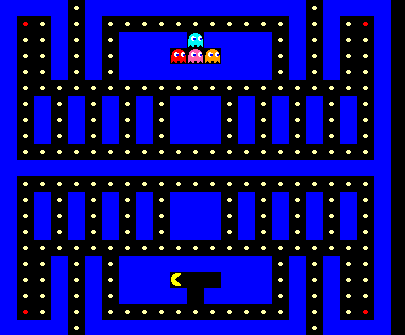
\includegraphics[scale=0.42]{ressources/block2}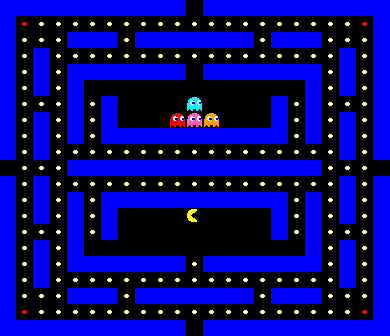
\includegraphics[scale=0.42]{ressources/block3}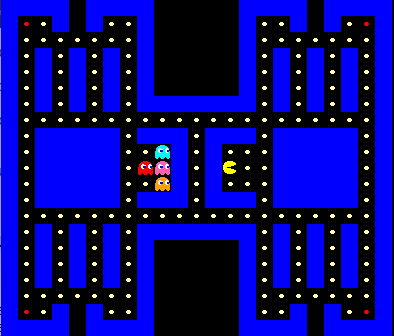
\includegraphics[scale=0.42]{ressources/block4}\caption{Différents labyrinthes disponibles}\label{figure1}


\end{figure}


\subsubsection{Sauvegarde de progression}
Au début de la partie, le programme demande le nom de l'utilisateur.
On vérifie ensuite s'il existe déjà un fichier de sauvegarde associé
à l'utilisateur, sinon on le crée. A chaque niveau est associé un
indice. On va stocker le plus grand indice des niveaux terminé par
le joueur dans le fichier de sauvegarde. A sa prochaine partie, si
l'utilisateur entre le même nom, et grâce aux boutons de changement
de niveau de l'interface, il pourra choisir le niveau qu'il désire
s'il l'a déjà débloqué.

Un design pattern Observer a été implémenté, par le biais de l'interface
GameObserver, afin de permettre de notifier le joueur par des pop-up
lorsque certains événements surviennent, tels que le fait de ne pas
pouvoir démarrer un niveau (car le joueur ne l'a pas débloqué), de
notifier le joueur de la fin de la partie et de sauvegarder sa progression.


\section{IA pour fantômes - Gallois Florent}
\subsection{Programme initial et objectifs}
Actuellement, les comportements des 4 fantômes du jeu Pac-man sont erratiques : 
leur trajectoire est déterminée aléatoirement.

Nous allons créer des IA pour les fantômes afin de leur donner des trajets plus intéressants pour le jeu.
Pour cela, l'objectif est d'affecter à chaque fantôme 2 modes : un mode de poursuite pendant lequel il suivra une stratégie de poursuite et un mode de dispersion pendant lequel il suivra une trajectoire bien définie.
Le mode poursuite ayant déjà été réalisé dans le logiciel,il ne nous reste à créer plus que le mode dispersion : 
Chaque fantôme doit régulièrement se rendre dans un coin : Pinky en haut à gauche, Blinky en haut à droite, Clyde en bas à gauche et enfin Inky en bas à droite.
Cependant, nous ne devons pas l'implémenter n'importe comment, mais nous devons réaliser un strategy design pattern afin d'implémenter le comportement des fantômes.
Un changement de stratégie permettra d'alterner entre la poursuite et la dispersion.
Ces alternements devront se faire suivant les périodes de temps indiqués dans le polycopié : 7 sec de dispersion puis 20 sec de poursuite, 7 sec de dispersion ... 

\subsection{Démarche suivie}
Le problème principal de cette réalisation est d'arriver à construire élégamment les IA des fantômes de tel sorte qu'un ajout de stratégie reste facile.
Comme il nous l'est suggéré, nous nous sommes intéréssées au strategy design pattern.

\begin{figure}[!h] %on ouvre l'environnement figure
		\centering
		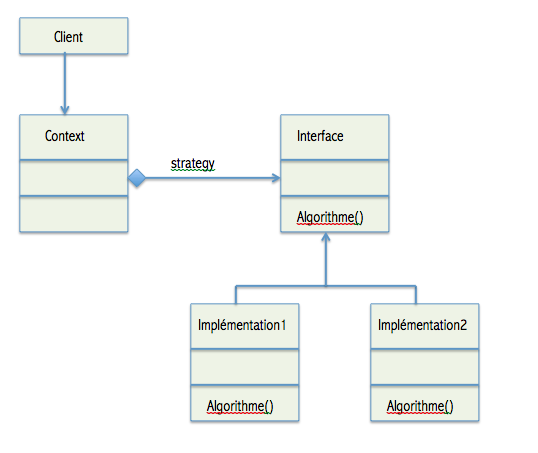
\includegraphics[scale=0.7]{ressources/StrategyDesignPattern.png}
		\caption{Design pattern strategy}\label{figure2}
\end{figure} 



Ce pattern est très utile lorsqu'il faut permuter dynamiquement des algorithmes.
Ou par exemple lorsque des classes ne diffèrent que par leur comportement. Ainsi, pour éviter de dupliquer le code, on crée une seule classe comportant les éléments de base ainsi qu'une interface implémentées par diverses classes décrivant les différents comportements de la classe centrale.

De prime abord, il a été pensé de créer pour chacun des fantômes, une interface qui était implémentée par 2 classes : une classe de poursuite et une classe de dispersion.
Or cela engendrait toujours du code dupliqué : les algorithmes de dispersion sont tous les mêmes.

Pour la première version du logiciel, un pattern comme celui qui suit a été crée :

\begin{figure}[!h] %on ouvre l'environnement figure
		\centering
		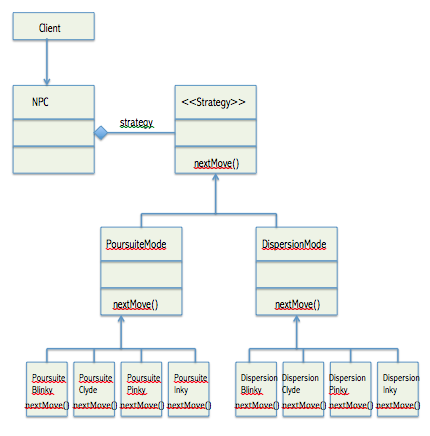
\includegraphics[scale=0.9]{ressources/StrategyDP.png}
		\caption{Design pattern strategy appliqué}\label{figure3}
\end{figure}


4 classes associées au mode poursuite pour chaque fantôme ont été crée dans lesquelles la méthode de poursuite a été copié collé. Ces 4 classes héritaient de la classe abstraite PoursuiteMode.
4 autres classes ont vu le jour représentant le mode dispersion de chaque fantôme.
Ces 4 classes héritaient de la classe abstraite DispersionMode.
Et enfin, PoursuiteMode et DispersionMode implémentaient l'interface Strategy.

Pour la 2ème version du logiciel, l'algorithme de dispersion a été crée.
Afin de pouvoir l'exécuter, des variables d'instance ont été aménagé dans la classe Ghost. Un string atteintHome indique si le fantôme a atteint sa case maison (la case du coin), un tableau de directions mémorise le chemin qu'il devra emprunter après avoir visité sa case maison. Un autre tableau de directions représente le chemin qu'il doit prendre à la prochaine occurence et enfin un square représentant sa case "maison".
Cet algorithme est placé dans la classe DispersionMode. Les classes filles font appel à cette même méthode.

La 3ème version, nous avons mis en place la variable strategy nous permettant de jongler entre la dispersion et la poursuite.
Ainsi, un String est placé dans la classe NPC représentant la stratégie en cours : ModeDispersion ou ModePoursuite. Lorsque la stratégie change,au cours du temps, cette variable est modifiée grâce à setStrategy.
Ainsi la méthode nextMove() de blinky par exemple appelle directement la méthode de sa classe de dispersion ou sa classe de poursuite associée en fonction de la valeur de cette variable.
Par conséquent, si l'on souhaite modifier la stratégie d'un fantôme, nous n'avons plus à changer le code dans toutes les classes fantômes mais à rectifier les appels aux méthodes.

Enfin, pour la 4ème et dernière version du logiciel, nous avons indiqué au programme de permuter entre les 2 stratégies en fonction du temps.
Dans la classe NpcMoveTask, une variable temps est crée pour suivre l'écoulement du temps. Celle-ci est incrémentée à chaque occurence de la fonction run de la moyenne d' intervalle entre 2 coups d'un fantôme. 
Dans la fonction run, en fonction de la valeur de cette variable, nous appelons la méthode setStrategy de la classe NPC afin de switcher la stratégie des fantômes.

\section{Difficultés liées au merge}
Pour la fusion entre la fonctionnalité "Supergomme" et la fonctionnalité "série de labyrinthe", nous n'avons eu aucun conflit et le jeu était en parfait état de marche avec les deux fonctionnalités en même temps.

Pour la fusion avec la troisième fonctionnalité, nous avons eu quelques conflits notamment dans les classes "MapParser" ainsi que dans les classe des fantômes (Blinky, Clyde, Inky et Pinky) mais cela s'est assez vite régler car nos codes étaient tout de même compatible.

\section{Analyse de la qualité du code}
\subsection{Outils utilisés}
\subsubsection{Google CodePro AnalitiX}
Le premier outil utilisé est Google CodePro AnalitiX, sous sa forme
plugin Eclipse.

Il s'agit d'un outil très complet qui permet le calcul des métriques,
la détection de code dupliqué, l'analyse des dépendances, la couverture
du code et des tests. Ici, nous l'utiliserons pour le calcul des métriques,
la détection de code dupliqué et l'analyse des dépendances.

\subsubsection{EclEmma}
Le second outil est Emma, sous sa forme plugin Eclipse (EclEmma).

Emma est un outils utilisé pour vérifier la couverture du code ainsi
que des tests lors de l'exécution de ces derniers.

\subsubsection{CodeCity}
Le troisième outil est CodeCity.

CodeCity est un outil qui permet de visualiser les métriques sous
forme graphique. Nous l'utiliserons pour constater les différences
entre le projet de base et le projet modifié.

\subsubsection{PMD}
Le dernier outils utilisé est PMD, sous sa forme plugin Eclipse.

PMD est un logiciel permettant de détecter les mauvaises pratiques
de programmation (``Bad Smells''). Nous regarderons la variation
de l'apparition de ces ``bad smells'' lors de la modification du
projet.

\subsection{Analyse des dépendances}
\subsubsection{Projet de base}
On peut voir sur la \hyperref[figure4]{Figure 4} un graphe des dépendances entre packages
du projet de base. On constate sur celui-ci qu'il y a beaucoup de
dépendances cycliques et que certaines classes ont une interdépendance
forte (par exemple ghost et level).

\begin{figure}[!h]
\begin{center}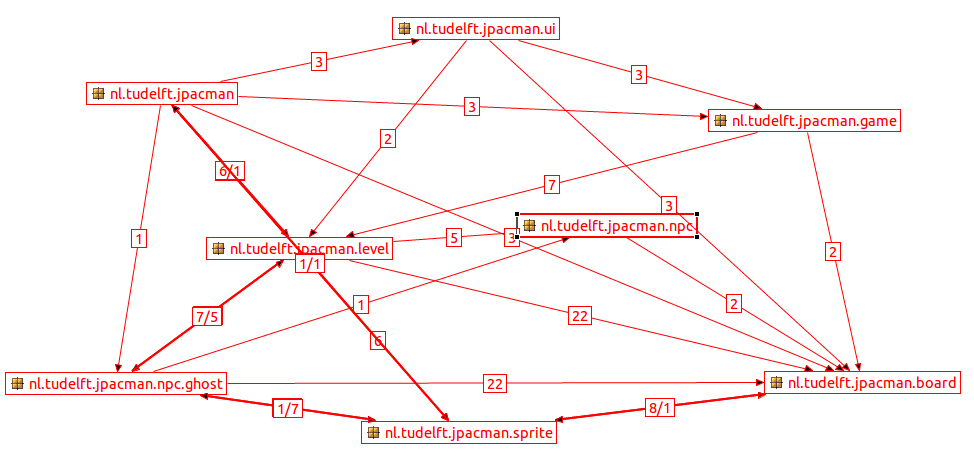
\includegraphics[scale=0.5]{ressources/final_initial_dependencies}\end{center}
\caption{Dépendances du projet de base}\label{figure4}
\end{figure}

\subsubsection{Projet modifié}
Un graphe des dépendances est représenté à la \hyperref[figure5]{Figure 5}, on peut constater
qu'en général les dépendances ont augmenté et que nous avons aussi
ajoutés des interdépendance entre deux packages qui n'en possédaient
pas.

\begin{figure}[!h]
\begin{center}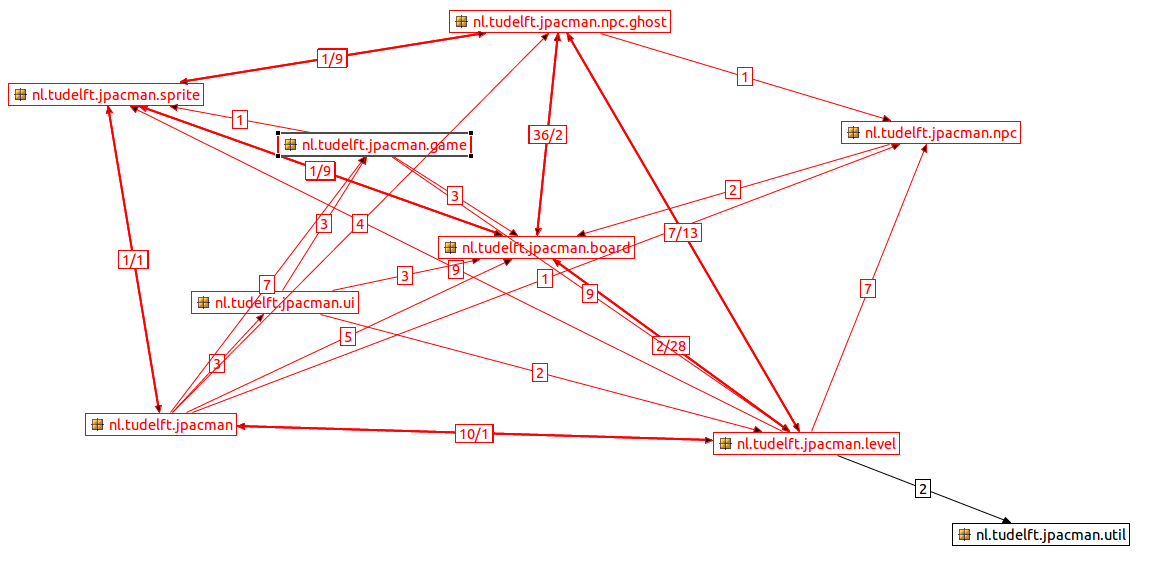
\includegraphics[scale=0.5]{ressources/final_new_dependencies}\end{center}\caption{Dépendances du projet modifié}\label{figure5}


\end{figure}

\subsection{Code dupliqué}
Selon Google CodePro AnalitiX, il y a 54 lignes de code dupliquées
dans le projet de base. Cette valeur est assez basse et montre la
volonté des développeurs du projet d'éviter la programmation ``copier-coller''

Google CodePro AnalitiX, pointe toujours 54 lignes de code dupliquées,
nous n'avons donc pas altéré ce point précis du code lors de nos modifications.


\subsection{Test \& Code Coverage}
\subsubsection{Projet de base}
EclEmma nous donne comme valeurs:
\begin{itemize}
\item test coverage : 80.9\%
\item code coverage (exécution sans jouer) : 41\%
\item code coverage (exécution partie type): $\sim$60\%
\end{itemize}

\subsubsection{Projet modifié}
EclEmma nous donne comme valeurs:
\begin{itemize}
\item test coverage : 71\%
\item code coverage (exécution sans jouer) : 35.9\%
\item code coverage (exécution partie type): $\sim$60\%
\end{itemize}
On peut constater que de manière générale le coverage a diminué, surtout
au niveau du test coverage. Bien qu'un paradigme de programmation
défensive à été utilisé, nous n'avons pas réussi à trouver de tests
qui couvrent l'entièreté du code ajouté.

\subsection{Métriques}
\subsubsection{Tableaux de métriques}
La \hyperref[figure6]{Figure 6} montre les deux tableaux de métriques côte à côte, ce
qui permet de comparer facilement les résultats.

On peux noter, entre autres, un légère augmentation de la complexité
cyclomatique, un accroissement général de la taille des différentes
classes (nombre de méthodes et nombre de lignes) et une légère diminution
du ratio de commentaires.

\begin{figure}[!h]
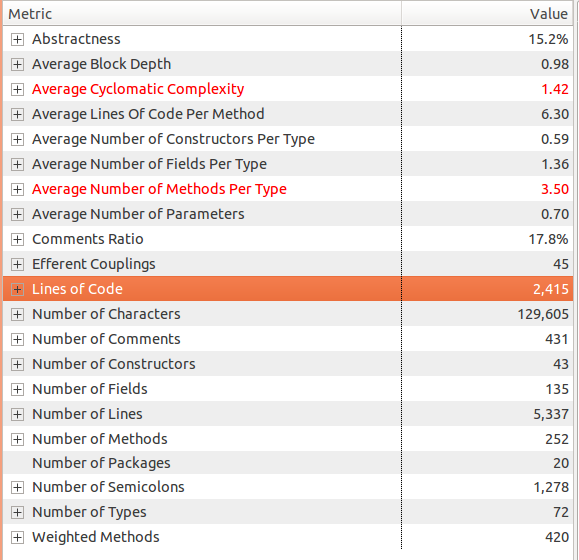
\includegraphics[scale=0.45]{ressources/final_initial_metrics}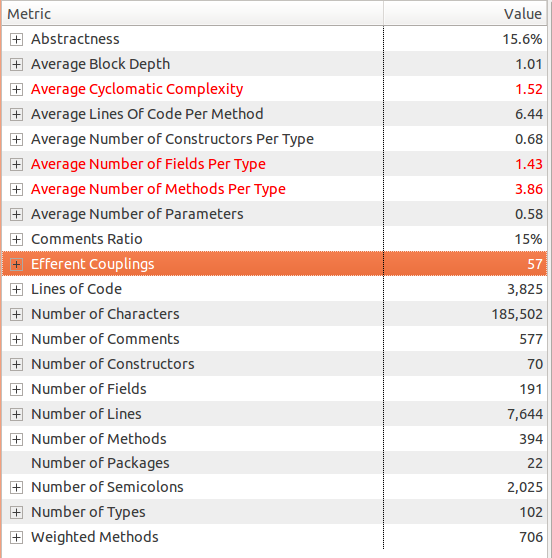
\includegraphics[scale=0.45]{ressources/final_new_metrics}\caption{Comparaison des tableaux de métriques (initial à gauche)}\label{figure6}


\end{figure}

\subsubsection{CodeCity : méthodes par classes}
Codecity nous permet de représenter graphiquement certaines métriques
par classes sur l'ensemble du projet.

Ici(\hyperref[figure7]{Figure 7}) nous nous intéressons au nombre de méthodes par classe, on voit
que, de manière générale, celui augmente pour l'ensemble du projet.

\begin{figure}[!h]
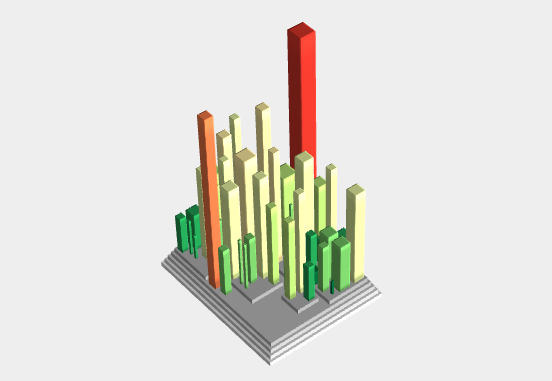
\includegraphics[scale=0.5]{ressources/final_initial_declared_methods}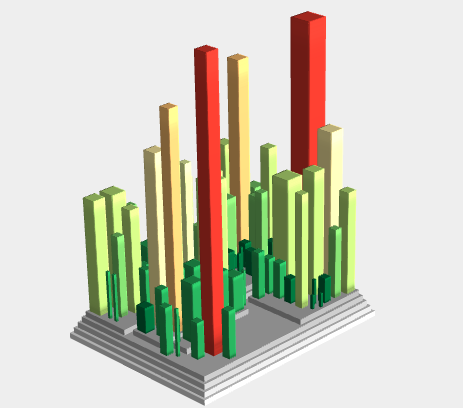
\includegraphics[scale=0.5]{ressources/final_new_declared_methods}\caption{Comparaison du nombre de méthodes par classe (initial à gauche)}\label{figure7}


\end{figure}

\subsubsection{CodeCity : complexité cyclomatique}
On voit sur la \hyperref[figure8]{Figure 8} que la complexité cyclomatique reste sensiblement
la même.

\begin{figure}[!h]
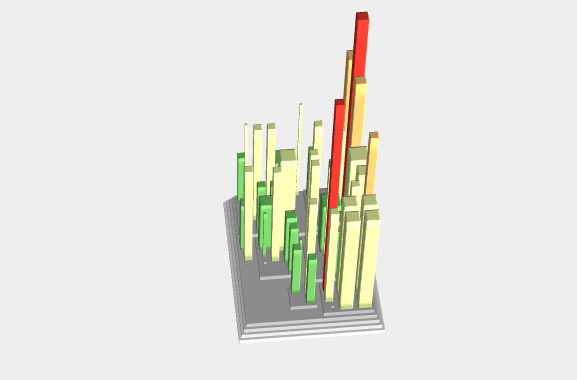
\includegraphics[scale=0.5]{ressources/final_initial_cyclomatic}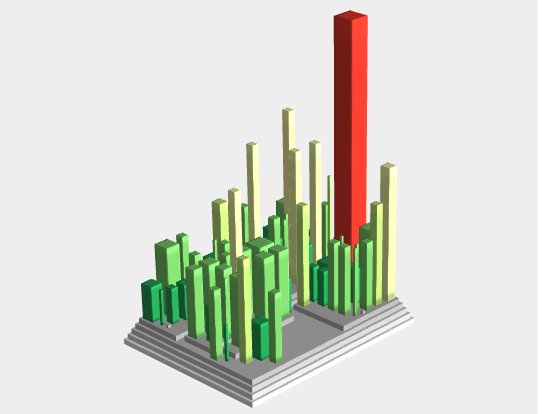
\includegraphics[scale=0.5]{ressources/final_new_cyclomatic}\caption{Comparaison de la complexité cyclomatique par classe (initial à gauche)}\label{figure8}


\end{figure}

\subsubsection{CodeCity : nombre de lignes de code}
Sur la \hyperref[figure9]{Figure 9} on peut voir que le nombre de lignes de codes par
classe est resté sensiblement identique, sauf pour deux d'entres elles
(Launcher et Level), qui mériteraient d'être séparée en plus petites
classes pour éviter le phénomène de ``God Class''.

\begin{figure}[!h]
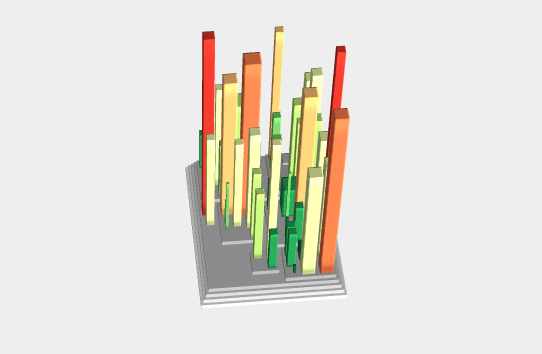
\includegraphics[scale=0.5]{ressources/final_initial_lines_of_code}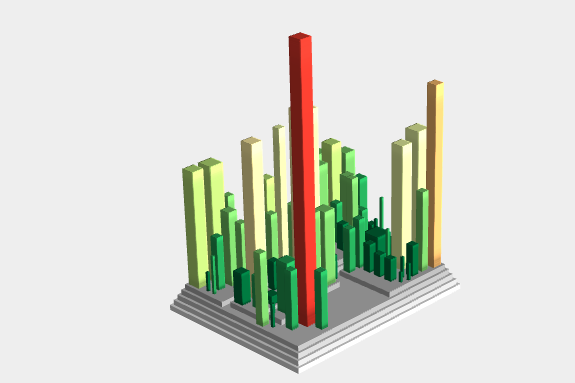
\includegraphics[scale=0.5]{ressources/final_new_lines_of_code}\caption{Comparaison du nombre de lignes de code par classe (initial à gauche)}\label{figure9}


\end{figure}

\subsection{Bad Smells}
PMD à mis en évidence 827 violations des bonnes pratiques de programmation
dans le projet initial. En ce qui concerne le projet final, on monte
à 1442 violations. Les erreurs les plus fréquentes sont ``variable
or argument could be final'' (39.6\% des violations pour le projet
initial contre 33\% pour le projet modifié) et ``law of demeter''
(10\% pour le projet initial contre 12\% pour le projet modifié) et
``short variable'' (10\% pour le projet initial contre 11\% pour
le projet modifié).

On a donc un accroisement de 74\% de violations selon PMD, à savoir
que le code est lui passé 2415 à 3825 lignes de code, c'est à dire
un accroissement de 58\% en ce qui concerne la taille du projet niveau
lignes de codes (lignes de code effectives, selon Google CodePro AnalitiX).
A noter aussi que PMD nous donne deux avertissements pour ``God Class''
pour les classes Level et Launcher, qui ont beaucoup crû pendant nos
modifications respectives. Il semble qu'un refactoring soit nécessaire
à ce niveau là pour pouvoir poursuivre la maintenance logicielle.

\end{document}